\documentclass[a4paper, 12 pt]{article}
\usepackage[utf8]{inputenc}
\usepackage[T1]{fontenc}
\usepackage[slovene]{babel}
\usepackage{lmodern}
\usepackage{amsmath}
\usepackage{amsfonts}
\usepackage{amssymb}
\usepackage{units}
\usepackage{eurosym}
\usepackage{pdfpages}
\usepackage{comment}
\usepackage{enumerate}
\usepackage{mathtools}
\usepackage{amsthm}
\usepackage{float}


% Matematicna okolja
\theoremstyle{definition}
\newtheorem*{definicija}{Definicija}
\newtheorem*{primer}{Primer}

\theoremstyle{plain}
\newtheorem*{lema}{Lema}
\newtheorem*{izrek}{Izrek}
\newtheorem*{trditev}{Trditev}
\newtheorem*{posledica}{Posledica}

\theoremstyle{remark}
\newtheorem*{opomba}{Opomba}


% ==============================================================
\begin{document}
\begin{titlepage}
		\begin{center}
		
		\large
		Univerza v Ljubljani\\
		\normalsize
		Fakulteta za matematiko in fiziko\\
		
		\small
		Finančna matematika - 1. stopnja\\
		
		\vspace{5 cm} 
		
		\large
		Matej Škerlep \\
		
		\vspace{0.5cm}
		\LARGE
		\textbf{Problem največje neodvisne množice}
		
		\vspace{0.5 cm}
		\normalsize
		Projekt pri predmetu finančni praktikum
		
		\vspace{1.5cm}
		\normalsize
		Mentorja: prof. dr. Riste Škrekovski in asist. dr. Janoš Vidali
		
		\vfill
		
		\large Ljubljana, 2020
		
		\end{center}
\end{titlepage}
% ==========================================================
\tableofcontents

\listoffigures

\listoftables
\newpage
% ==========================================================
\section{Dodatek} % ============================================

\section{Analiza algoritmov na Petersenovem grafu}
V nadaljevanju sem se odločil izvesti tudi algeoritme na Petersenovem grafu.


\begin{figure}[H]
\centering
  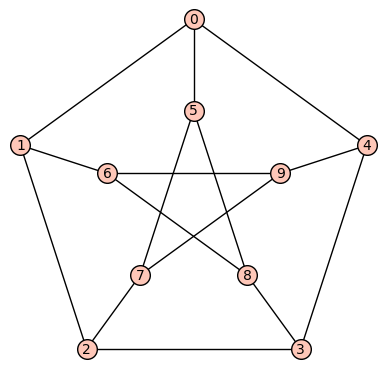
\includegraphics[scale=0.28]{Petersenov graf.png}
  \caption{Petersenov graf}
\end{figure}

CLP in lokalno iskanje vedno najdeta enako moč največje neodvisne množice, medtem ko so vozlišča v njej enaka le v 10 odstotkih poskusov. Relaksacija CLP pa vedno vrača prazno množico. Časovne zahtevnosti in moči množice $I$ so podane v spodnji tabeli.

\begin{table}[H]
\centering
\begin{tabular}{|p{3cm}|p{2.7cm}|p{4.7cm}|}
\hline
\textbf{Algoritem}  & \textbf{Moč množice $I$} & \textbf{Čas izvedbe algoritma} \\ \hline
CLP    & 4 &  		   0.0106859 $s$\\ \hline
Relaks. CLP    & 0  &  0.0023558 $s$   \\ \hline
Lokalno iskanje & 4 &  0.0069702 $s$ \\ \hline
\end{tabular}
\caption{Moč množice I in časovna zahtevnost iskanja na Petersenovem grafu}
\label{fig:petersenov} 
\end{table}

\section{Analiza algoritmov na hiperkockah}
Pri analizi vseh treh algoritmov na hiperkockah sem pogledal največje množice neodvisnih vozlišč grafa in časovne zahtevnosti algoritmov na hiperkockah na 4, 8, 16, 32, 64 in 128 vozliščih. 

\begin{table}[H]
\centering
\begin{tabular}{|p{3cm}|p{1cm}|p{2.7cm}|p{3.2cm}|}
\hline
\textbf{Število vozlišč}  & \textbf{CLP} & \textbf{Relaks. CLP} & \textbf{Lokalno iskanje} \\ \hline
4     & 2 &2  &2  \\ \hline
8     & 4 & 4 &4  \\ \hline
16   & 8 & 8  &8  \\ \hline
32   & 16 &16  &16  \\ \hline
64   & 32 & 32 &  32 \\ \hline
128 & 64 & 64 & 64  \\ \hline
\end{tabular}
\caption{Moč množice $I$ na hiperkockah}
\label{fig:hipekocka I} 
\end{table}
Vidimo, da so vse tri množice $I$ ves čas enake in je njihova moč enako ravno polovico števila vseh vozlišč grafa. To je seveda logično, saj gre za dvodelen graf. 

%% naredi tle še graf za časovno zahtevnost

\section{Zaključek}


% ==========================================================
\end{document}